\section{Tainting dependencies}
\label{sect:impl:tainting_deps}
``Tainting dependencies'' is a method of translating XQuery queries to
relational algebra. The semantics of this method is described in detail
throughout chapter \ref{sect:translation}. This section
describes an implementation of a subset of the rules in this method -- an
implementation which is capable of translating simple FLWOR expressions,
sequences, and variables.

\subsection{FLWOR expressions}
The translation process for FLWOR expressions was outlined in section
\ref{sect:trans:TD:simpleFLWOR}. Consider inference rule
\ref{rule:trans:TD:forbind} on page \pageref{rule:trans:TD:forbind}. This
inference rule states how to translate and bind an iterator variable in a
for-clause in a FLWOR expressions. First a for-clause is visited, and the
child is flagged as a FLWOR tuplet definition:

\begin{Verbatim}
public TraverseReturn visitAST_FORCLAUSE(XQFTTree tree) {

    ((XQFTTree)tree.getChild(0)).setFlworTupleDef(true);
    acceptThis(tree.getChild(0));
    return null;
}
\end{Verbatim}

Next a dollar sign is visited (which carries the meaning of a variable in the
abstract syntax tree). If the child count is more than one, it is an
assignment. Note that the \texttt{isIterationVar} flag is \textit{true} if
this assignment is a tuple definition as flagged earlier. Then, if this is an
assignment and a tuple definition, the right-hand side of the assignment is
translated, and the symbol is entered into a symbol table. Note that the
creation of the project operator is required by inference rule
\ref{rule:trans:TD:forbind}:

\begin{Verbatim}
public TraverseReturn visitDOLLARSi(XQFTTree tree) {
      
    boolean isIterationVar = tree.isFlworTupleDef();
      
    String varName = tree.getChild(0).getText();
      
    // Assignment?
    if (tree.getChildCount() > 1) {
         
        // Visit children on the right side of the assignment
        TraverseReturn tr = acceptThis(tree.getChild(1));
          
        // Required for tainting deps method
        Project project = new Project(
            "[" + varName + "numb, value]", 
            tr.getOperatorTree());

        // Assign metadata
        tr.setOperatorTree(project);
        tr.setSingleton(true);
          
        // Enter into symbol table
        SymTabEntry tmp = Scope.set(tree.getChild(0).getText(), 
                              tr, isIterationVar);
          
        if (isIterationVar) {
           Scope.getInstance().setCurrentIterVar(
                                   new VarRef(tmp.getName()));
        }
          
        return tr;
    }

    .
    .
    .
\end{Verbatim}

This example can be better understood if seen in context of an abstract syntax
tree example. Considering the example in figure \ref{fig:impl:td:flwor2}. Here
the \textit{AST\_FORCLAUSE} node will be visited by the
\texttt{visitAST\_FORCLAUSE()} method in the visitor and the
\texttt{isFlworTupleDef} flag will be set to \textit{true}. Then the variable
node (the dollar sign) will be visited by the \textit{visitDOLLARSi()} method,
and the translation of the for-clause is completed.

\begin{figure}[!htp]
\begin{center}
  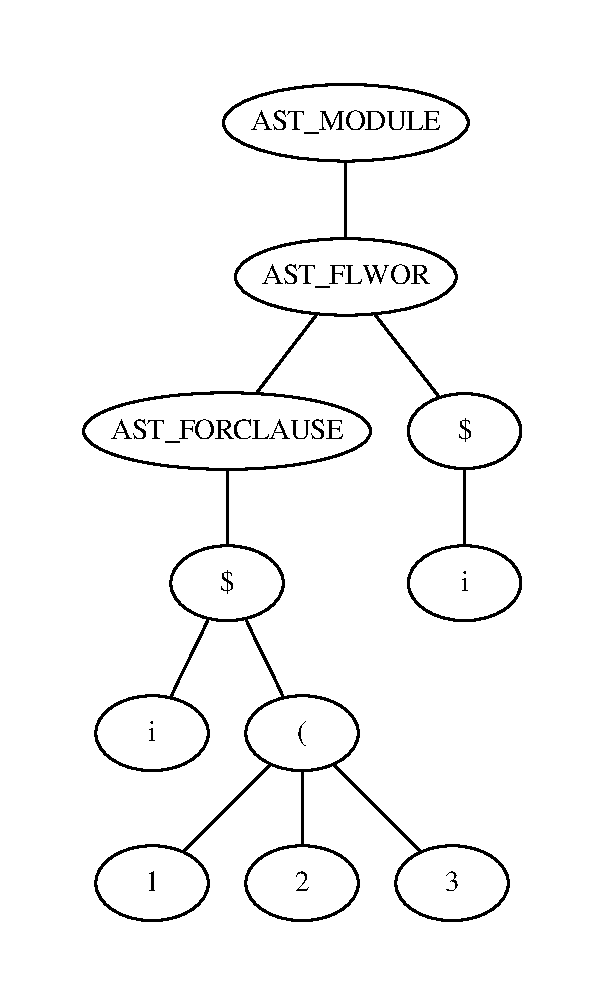
\includegraphics[scale=0.4]{img/graphs/flwor2}
  \caption{FLWOR syntax tree example}
  \label{fig:impl:td:flwor2}
\end{center}
\end{figure}

Following the translation of the for-clause, the return clause is translated in
a similar manner. However this translation is slightly more complicated. The
translation is dependent on whether the return clause contains code which
references the current iteration variable. If this is the case, then a
translation which applies tainting given by the rule in figure
\ref{eq:trans:TD:taint} on page \pageref{eq:trans:TD:taint} must be used. In
particular, the rule in figure \ref{rule:trans:TD:returnTaint} shown on page
\pageref{rule:trans:TD:returnTaint} must be applied (which implies the former
rule):

\begin{Verbatim}
// Sort and partition fields
String[] sortBy = {Scope.getInstance().getCurrentIterVar().getName() 
		          + "numb", "index"};
String[] partitionBy 
	= new String[returnClauseResult.getVarRefs().size() - 1];

// Calculate variable references
VarRefSet prevVarRefs 
	= (VarRefSet)returnClauseResult.getVarRefs().clone();         
prevVarRefs.remove(Scope.getInstance().getCurrentIterVar());

int i = 0;
for (VarRef ref : prevVarRefs) {
    partitionBy[i] = ref.getName();
    i++;
}

// Construct MQL
Numberate numberate = new Numberate("index", 
                                    sortBy, 
                                    partitionBy, 
                                    returnClauseResult.getOperatorTree());

// Construct result
TraverseReturn result = new TraverseReturn();
result.setSingleton(false);
result.setVarRefs(returnClauseResult.getVarRefs());
result.setOperatorTree(numberate);

// Remove current iter var from varrefs
result.getVarRefs().remove(Scope.getInstance().getCurrentIterVar());

Scope.pop();
return result;
\end{Verbatim}

Note that the code in this example is executed if and only if
there is a reference to the iteration variable in the return clause.

If there is no reference to the current iteration variable, then the
translation is performed as a regular XQuery translation without tainting.

\subsection{Sequences}
\label{sect:impl:td:seq}
The translation process for sequence construction is described in section
\ref{sect:trans:TD:seqBuild}. This rule is somewhat complex, and requires
collecting all variable references from all children before performing the
actual translation. Furthermore, for any variable reference in a left-most
child, this variable reference must taint all right-most children:

\begin{Verbatim}
for (TraverseReturn childResult : childResults) {
    VarRefSet varRefsDiff;
    Operator expr = childResult.getOperatorTree();
    
    VarRefSet tmp = childResult.getVarRefs();
    varRefsDiff = (VarRefSet)varRefs.clone();
    varRefsDiff.removeAll(tmp);

    for (VarRef varRef : varRefsDiff) {
        Project project = new Project(varRef.getName() + "numb", 
                Scope.get(varRef.getName()).getTraverseReturn().getOperatorTree());
        
        Cross cross = new Cross(project, expr);
        expr = cross;
     }

    if (childResult.isSingleton()) {
        expr = new Project("sprIdx="+(c+1)+",index,value", expr);
    }
    else {
        expr = new Project("sprIdx="+(c+1)+",value", expr);
    }
    operators.add(expr);
    c++;
}
\end{Verbatim}

This will propagate tainting throughout the siblings as required. When this
procedure is complete, the operators (in the \texttt{operators} list) are
added as children to a \textsf{union()} operator, and then a
\textsf{numberate()} operator. This completes the translation of a sequence
constructor.

Note that the parantheses in sequence expressions are not required, and
according to specification, sequence expressions are recognised by the comma
symbols and not parantheses. However, the XQFT Parser rewrites sequence
expressions into including a paranthesis as start token for sequence subtrees
within the AST.

\subsection{If-then-else}
The translation process for conditional expressions is explained in section
\ref{sect:trans:TD:ifThenElse}. In particular, rule
\ref{rule:trans:TD:conditional} describes this translation. 

First the child expressions are visited:

\begin{Verbatim}
// if (e1) then e2 else e3
XQFTTree e1 = (XQFTTree)tree.getChild(0); 
XQFTTree e2 = (XQFTTree)tree.getChild(1);
XQFTTree e3 = (XQFTTree)tree.getChild(2);
        
// Visit the expressions
TraverseReturn r_e1 = acceptThis(e1);
TraverseReturn r_e2 = acceptThis(e2);
TraverseReturn r_e3 = acceptThis(e3);
\end{Verbatim}

The variables \texttt{e1},\texttt{e2}, and \texttt{e2} correspond to the
expressions $e_1$,$e_2$, and $e_3$ in rule \ref{rule:trans:TD:conditional},
while \texttt{r\_e1},\texttt{r\_e3}, and \texttt{r\_e3} correspond to
\textbf{r}($e_1$), \textbf{r}($e_2$), and \textbf{r}($e_3$).

Continuing, sets of variable references (iterator dependencies) are obtained:
         
\begin{Verbatim}
// VarRefs: e2 u e3
VarRefSet v_e2_u_e3 = (VarRefSet)r_e2.getVarRefs().clone();
v_e2_u_e3.addAll(r_e3.getVarRefs());

// VarRefs: (e2 u e3) n e1
VarRefSet v_e2_u_e3_n_e1 = (VarRefSet)v_e2_u_e3.clone();
v_e2_u_e3_n_e1.retainAll(r_e1.getVarRefs());

// VarRefs: e1 u e2 u e3
VarRefSet v_e1_u_e2_u_e3 = (VarRefSet)r_e1.getVarRefs().clone();
v_e1_u_e2_u_e3.addAll(r_e2.getVarRefs());
v_e1_u_e2_u_e3.addAll(r_e3.getVarRefs());
\end{Verbatim}

If not completely clear, the variable \texttt{v\_e2\_u\_e3} corresponds to
$e_2 \cup e_3$, \texttt{v\_e2\_u\_e3\_n\_e1} corresponds to $(e_2 \cup e_3) \cap
e_1$, and \texttt{v\_e1\_u\_e2\_u\_e3} corresponds to $e_2 \cup e_3 \cup
e_1$.

This result is used to create the to \textsf{project()} operators and union
them together:

\begin{Verbatim}
// Alternatives
Project project_alt1 = new Project("index, alt=1, " + 
                       v_e2_u_e3.toStringList() + 
                       ", value", 
                       this.taint(r_e2, r_e3.getVarRefs())
                           .getOperatorTree()); 

Project project_alt2 = new Project("index, alt=2, " +
                        v_e2_u_e3.toStringList() + 
                        ", value", 
                        this.taint(r_e3, r_e2.getVarRefs())
                            .getOperatorTree()); 

// Union
Union union = new Union(null, null);
union.addOperator(project_alt1);
union.addOperator(project_alt2);
\end{Verbatim}

The translation is finalised by using this result to construct a join and apply
the \textsf{select()} operator:

\begin{Verbatim}
// HHjoin
HHJoin hhjoin = new HHJoin("[" + 
                v_e2_u_e3_n_e1.toStringList() + "],
                [" + v_e2_u_e3_n_e1.toStringList() + "], 
                [index = l.index, " + 
                v_e1_u_e2_u_e3.toStringList() +
                ", lvalue = l.value, rvalue = r.value]", 
                union, r_e1.getOperatorTree());

// Select
Select select = new Select("ifthenelse(xqBoolean(rvalue), 
                    eq(alt,1), eq(alt,2))", hhjoin);

// Project
Project project = new Project("index, " + 
                  v_e1_u_e2_u_e3.toStringList() +
                  ", value = lvalue" , select);
\end{Verbatim}
